\section{Introduction}
\label{sec:intro}

Data have become a defining production factor of the digital economy \cite{jones2020}. Unlike physical capital, data are non-rival: the same record can be reused across products, algorithms, and decisions without being depleted \cite{farboodi2020}. Their marginal replication cost is close to zero, so marginal cost provides little guidance for valuation \cite{bergemann2019}. Data are also rarely traded in transparent secondary markets, and their value is bundled with algorithms, platforms, and customer relationships \cite{oecd2022}. These features make firm-level data assets difficult to price.

Privacy regulation offers a way to observe the value of one class of data. The European Union's General Data Protection Regulation raised the cost of collecting and using personal data \cite{goldberg2024}. Apple's App Tracking Transparency (ATT) policy required user permission before cross-app tracking \cite{apple2020}. China's Personal Information Protection Law (PIPL) imposed consent, minimization, and sharing rules on personal information \cite{pipl2021}. A growing literature documents the effects of these regimes on e-commerce \cite{aridor2024}, app monetization \cite{kesler2023}, and the app ecosystem \cite{cheyre2024}.

Existing studies focus on average effects on outcomes. They do not measure how the value loss varies with a firm's ex ante dependence on third-party data. This distinction matters because digital firms differ sharply in their data architecture: some own logged-in users, transaction histories, and first-party applications, whereas others rely on external data purchases, cross-app identifiers, and platform traffic. A privacy shock should therefore have heterogeneous valuation effects even when it applies to all firms at the same time.

Measuring these differences is difficult because data use is not reported in financial statements. Text provides an alternative \cite{gentzkow2019}. Annual reports describe business models, traffic acquisition, advertising, data partnerships, and platform dependence \cite{loughran2011}. Dictionary-based text measures have been used to study policy uncertainty \cite{baker2016}, digital transformation \cite{jin2026}, and corporate disclosure \cite{loughran2011}. Building on this approach, we construct a Third-Party Data Dependency Index (TDDI) from the 2019 annual reports of Chinese A-share digital firms.

The TDDI covers four dimensions: third-party data acquisition, third-party traffic and advertising, user tracking and targeting, and platform dependence. We validate the index with split-half reliability, industry patterns, and a placebo index of generic digitalization. The index is predetermined relative to the 2021 privacy shock. This timing avoids the concern that firms adjust their disclosure in response to the regulation.

We combine the TDDI with a firm-quarter panel of 298 Chinese A-share digital firms from 2018Q1 to 2023Q4. We estimate difference-in-differences (DiD) models with firm and industry-by-quarter fixed effects \cite{dechaisemartin2020}. We report dynamic event studies \cite{rambachan2023}, dose-response bins \cite{callaway2024}, placebo dates, and wild cluster bootstrap inference \cite{mackinnon2017}. Identification rests on the timing of the privacy regime and on cross-sectional variation in pre-shock TDDI.

High-TDDI firms experience a 9.2\% relative decline in log Tobin's Q and a 2.45 percentage-point decline in gross margin after the shock. ROA and selling-expense ratios do not change significantly. The effect is concentrated in B2B data-service firms; consumer internet firms are not significantly affected. The implied market-value loss for high-exposure firms is RMB 203.7 billion, with a 95\% confidence interval of RMB 54.7--352.8 billion.

The paper makes four contributions. First, it provides a replicable, predetermined measure of third-party data dependence \cite{gentzkow2019}. Second, it estimates the valuation effect of a privacy-regime shock using a continuous exposure design \cite{aridor2024}. Third, it documents a B2B--B2C difference that is invisible in industry-average estimates \cite{chen2026}. Fourth, it translates the coefficient into a data risk exposure that can inform data-asset accounting and privacy policy \cite{ma2025}.

The research objectives are threefold. The first is to measure firm-level third-party data dependence from public disclosures. The second is to estimate how this dependence affects valuation and operating outcomes under the 2021 privacy regime. The third is to translate the estimates into an industry-level data risk exposure that can inform data-asset accounting and privacy policy.

The paper connects three literatures. The first treats data as an economic asset \cite{jones2020}. It emphasizes non-rivalry \cite{farboodi2020} and the market for information \cite{bergemann2019}. The second studies privacy and personalized markets \cite{acquisti2016}. It examines how consumers respond to tracking \cite{tucker2014} and how firms price privacy \cite{johnson2020}. The third uses text to measure firm-level digital and data characteristics \cite{gentzkow2019}. It also speaks to recent work in this journal on privacy regulation \cite{chen2026,li2026,kang2025,lin2021,zhang2026} and on the marketization of data elements in China \cite{jin2026,ma2025,song2025}.

The remainder of the paper proceeds as follows. Section 2 reviews the literature. Section 3 develops the theoretical analysis and states the hypotheses. Section 4 describes the institutional setting. Section 5 presents the data and sample. Section 6 constructs and validates the TDDI. Section 7 explains the empirical strategy. Section 8 reports the baseline results. Section 9 examines mechanisms and heterogeneity. Section 10 estimates the data risk exposure. Section 11 discusses implications, and Section 12 concludes.

\begin{figure}[H]
\centering
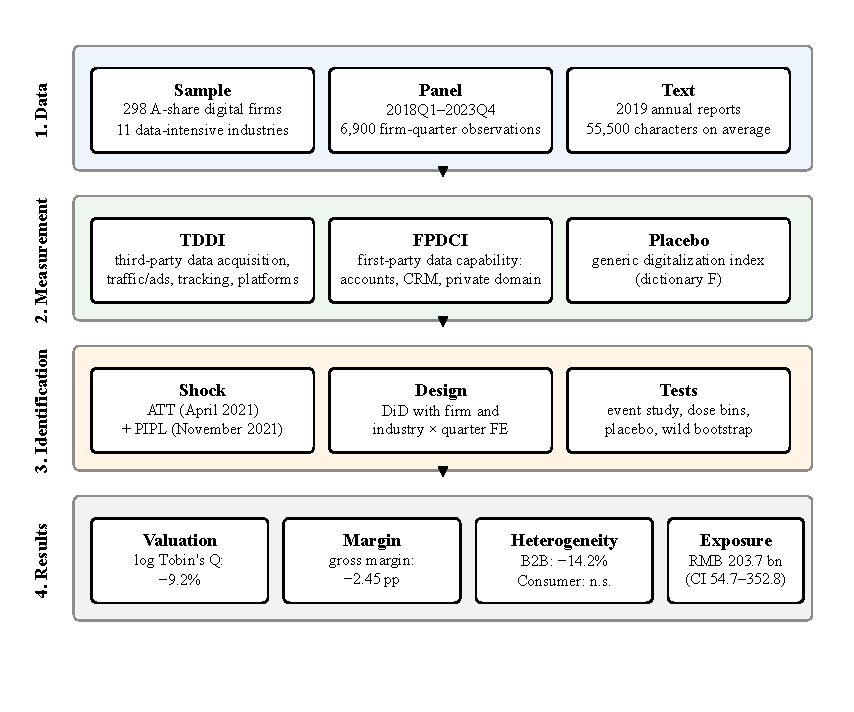
\includegraphics[width=0.95\textwidth]{fig0_framework.pdf}
\caption{Research framework. The figure summarizes the data, measurement, identification, and valuation steps. TDDI denotes the Third-Party Data Dependency Index; FPDCI denotes first-party data capability; DiD denotes difference-in-differences.}
\label{fig:framework}
\end{figure}
